\documentclass[12pt, letterpaper,notitlepage]{article}
\usepackage[utf8]{inputenc}
\usepackage{natbib}
\usepackage{setspace}
\usepackage{fullpage}
\usepackage{graphicx}
\usepackage[export]{adjustbox}
\usepackage{caption}
\usepackage{subcaption}
\usepackage[hidelinks]{hyperref}
\usepackage{array}
\usepackage{multirow}
\usepackage{tabularx}
\usepackage{rotating}
\usepackage[svgnames]{xcolor}
\usepackage{listings}
\usepackage{xcolor}
\usepackage{titling}
\usepackage[
type={CC},
modifier={by},
version={4.0},
]{doclicense}



\definecolor{light-gray}{gray}{0.95}

\lstset{language=R,
    basicstyle=\small\ttfamily,
    stringstyle=\color{DarkGreen},
    %otherkeywords={read_dta},
    %morekeywords={TRUE,FALSE},
    %deletekeywords={data,frame,length,as,character},
    %keywordstyle=\color{blue},
    backgroundcolor = \color{light-gray},
    commentstyle=\color{DarkGreen},
}


%otherkeywords=0,1,2,3,4,5,6,7,8,9,

\renewcommand\maketitlehooka{\null\mbox{}\vfill}
\renewcommand\maketitlehookd{\vfill\null}

\begin{document}

\title{Survey Data Analysis R \\ Reference Guide}
\author{
  David J. Barney \\
    {\small\texttt{davidjbarney@gmail.com}} \\
      {\small\texttt{@davidjbarney}}
}
\date{Draft as of \today}


\begin{titlingpage}




\maketitle
\doclicenseThis
\end{titlingpage}


\newpage

\tableofcontents

\newpage


\section{Reading \& Exploring Data}


To read in your data:

\begin{lstlisting}
# Comma delimited format
dat <- read.csv("~/your/file/path")
# Tab delimited format
dat <- read.table("~/your/file/path")
# Stata (.dta) format
library(haven)
dat <- read_dta("~/your/file/path")
\end{lstlisting}


To view observations or summaries of a variable:

\begin{lstlisting}
# Print the top few observations of a variable
head(dataframe$vector)
# Print the bottom few observations of a variable
tail(dataframe$vector)
# Print all observations of a variable
print(dataframe$vector)
# Access a summary of a variable or model
summary(dataframe$vector)
summary(model)
\end{lstlisting}

To learn the structure or format of your data:

\begin{lstlisting}
# Access the type / storage mode of the data
typeof(dataframe$vector) 
# Access the structure of the data
str(dataframe) 
str(dataframe$vector) 
# Access the length of a vector (e.g. the number of observations)
length(dataframe$vector)
# Access the attributes and metadata of an object
attributes(dataframe) 
attributes(dataframe$vector) 
\end{lstlisting}

\newpage
\section{Manipulating Data}
\subsection{Recoding Data}
To recode values in base R:

\begin{lstlisting}
#Create a new vector to work with
cces16$ban_ar <- cces16$CC16_330d
#Attitudes toward gun control
#Call all values for "oppose" and replace with zero
cces16$ban_ar[cces16$ban_ar==2] <- 0
#Call all values for skipped / not asked and replace with missing
cces16$ban_ar[cces16$ban_ar==8] <- NA
cces16$ban_ar[cces16$ban_ar==9] <- NA
\end{lstlisting}

To collapse categories of an ordinal variable in base R:
\begin{lstlisting}
#Create a new vector to work with
cces16$pid <- cces16$pid7
#Recode values to missing
cces16$pid[cces16$pid==98] <- NA
cces16$pid[cces16$pid==99] <- NA
cces16$pid[cces16$pid==8] <- NA
#Collapse the categories
cces16$pid[cces16$pid==2] <- 1
cces16$pid[cces16$pid==3] <- 1
cces16$pid[cces16$pid==4] <- 2
cces16$pid[cces16$pid==5] <- 3
cces16$pid[cces16$pid==6] <- 3
cces16$pid[cces16$pid==7] <- 3
\end{lstlisting}

To cut a continuous variable into an ordinal one in base R:
\begin{lstlisting}
cces16$agecats <- cut(cces16$age,
                      breaks=c(-Inf, 35, 50, Inf),
                      labels=c("35 and Under","36 to 50","Over 50"))
\end{lstlisting}

To flip the direction of coding in base R:
\begin{lstlisting}
#Flip the coding
cces16$pid_reverse <- 4 - cces16$pid
\end{lstlisting}

To apply labels to factor levels of a recoded variable:
\begin{lstlisting}
cces16$pid_reverse <- factor(cces16$pid_reverse,
                             levels = c(1,2,3),
                             labels = c("Republican", "Independent",
                             "Democrat"))
\end{lstlisting}


\newpage

\subsection{Merging Data}
To merge data that have one common vector with the same name:


\begin{lstlisting}
library(haven)
cces16 <- read_dta("~/your/filepath/here")
cces16s <-  read.delim("~/your/filepath/here")
#Merge the primary and supplemental data by respondent state
cces16c <- merge(cces16, cces16s)
\end{lstlisting}

To merge data that have a common vector with different names:

\begin{lstlisting}
#Merge by state with different column names
cces16c <- merge(cces16, cces16s,
                 by.x = "inputstate", 
                 by.y = "inputstate")
\end{lstlisting}


\newpage

\section{Descriptive Statistics}
\subsection{Summary Statistics}
To summarize a variable:

\begin{lstlisting}
summary(cces16$age)
   Min. 1st Qu.  Median    Mean 3rd Qu.    Max. 
  18.00   33.00   49.00   47.88   61.00   99.00 
\end{lstlisting}


To call specific summary statistics:

\begin{lstlisting}
#Mean
mean(cces16$age)
#Standard deviation
sd(cces16$age)
#Minimum
min(cces16$age)
#Maximum
max(cces16$age)
#Range
range(cces16$age)
#Quantiles
quantile(cces16$age)
\end{lstlisting}

\subsection{Tabulations \& Cross Tabulations}

To tabulate a variable:
\begin{lstlisting}
# Tabulate PID
prop.table(table(cces16$pid_reverse))
 Republican Independent    Democrat 
  0.3336641   0.1679444   0.4983915 
\end{lstlisting}

To cross-tabulate two variables:
\begin{lstlisting}
# Tabulate PID by age categories
pidxage <- table(cces16$pid_reverse, cces16$agecats)
pidxage
prop.table(pidxage,2)
              35 and Under  36 to 50   Over 50
  Republican     0.2613407 0.3150328 0.3868747
  Independent    0.1708327 0.1874692 0.1569152
  Democrat       0.5678266 0.4974981 0.4562101
\end{lstlisting}

\newpage
\subsection{Summary Statistics by Group}
To summarize variables by group in base R:

\begin{lstlisting}
#Create a dataframe of the variables of interest
subgroup_vars <- c("age","pid")
subgroup_matrix <- as.matrix(cces16[subgroup_vars])
subgroup_df <- as.data.frame(subgroup_matrix)
aggregate(subgroup_df$age, list(subgroup_df$pid), mean)

  Group.1        x
1       1 46.58152
2       2 46.97732
3       3 51.23725
\end{lstlisting}

To summarize variables by group with \texttt{dplyr}:

\begin{lstlisting}
library(dplyr)
subgroup_means <- subgroup_df %>%
  group_by(pid) %>%
  summarise(mean = mean(age))
subgroup_means

# A tibble: 4 x 2
    pid  mean
  <dbl> <dbl>
1     1  46.6
2     2  47.0
3     3  51.2
4    NA  38.4
\end{lstlisting}

\newpage

To visualize subgroup means with \texttt{ggplot}:

\begin{lstlisting}
pid_labels <- c("Democrat", "Independent", "Republican")
sg_bp <- ggplot(subgroup_means, aes(y=mean, x=pid)) + 
  geom_bar(fill="lightskyblue",stat="identity") +
  #xlab("Partisanship") +
  ylab("Mean Age") +
  scale_x_discrete(name = "Partisanship",
                   limits=pid_labels)
sg_bp + coord_cartesian(ylim=c(45,55))
\end{lstlisting}

\begin{figure}[!ht]
\caption{\textsl{Bar Plot of Mean Age by Partisanship}}\label{fig:age_bp_sg}
\centering
  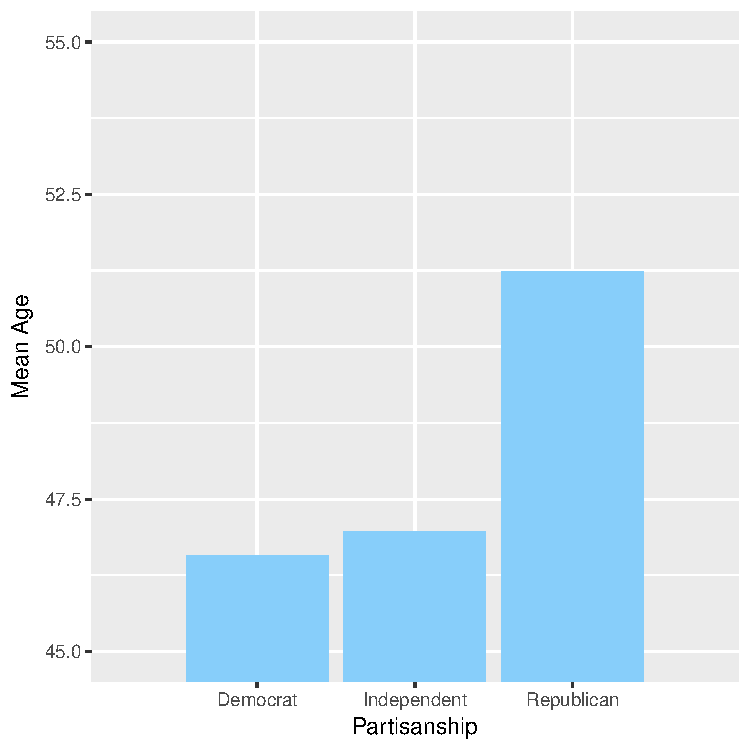
\includegraphics[width=.6\linewidth]{age_sg_bp.pdf}
\end{figure}

\clearpage

\subsection{Distributions}
To plot a histogram of a variable's distribution using \texttt{ggplot2}:

\begin{lstlisting}
#Histogram for age
library(ggplot2)
age_matrix <- as.matrix(cces16$age)
age_df <- as.data.frame(age_matrix)
ggplot(data = age_df, aes(x=age_df)) +
  geom_histogram(binwidth = 1) + 
  xlab("Age of Respondent") +
  ylab("Frequency")
#Density plot
ggplot(data = age_df, aes(x=age_df)) +
  geom_density(fill="lightblue") +
  xlab("Age of Respondent") +
  ylab("Density")
\end{lstlisting}

\begin{figure}[!ht]
\caption{Plotting Variable Distributions}
\centering
\begin{subfigure}{.5\textwidth}
  \centering
  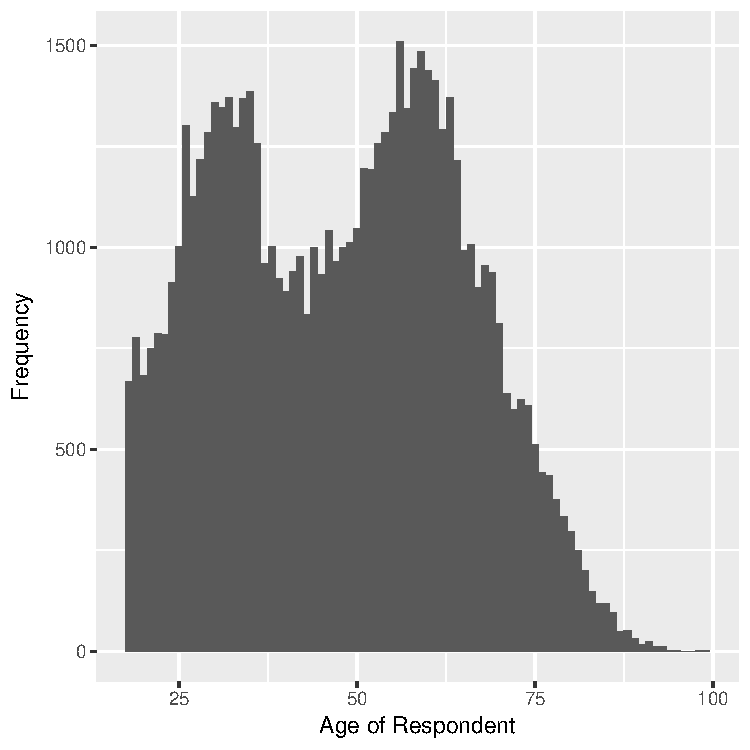
\includegraphics[width=.9\linewidth]{age_histogram.pdf}
  \caption{Histogram}
  \label{fig:sub1}
\end{subfigure}%
\begin{subfigure}{.5\textwidth}
  \centering
  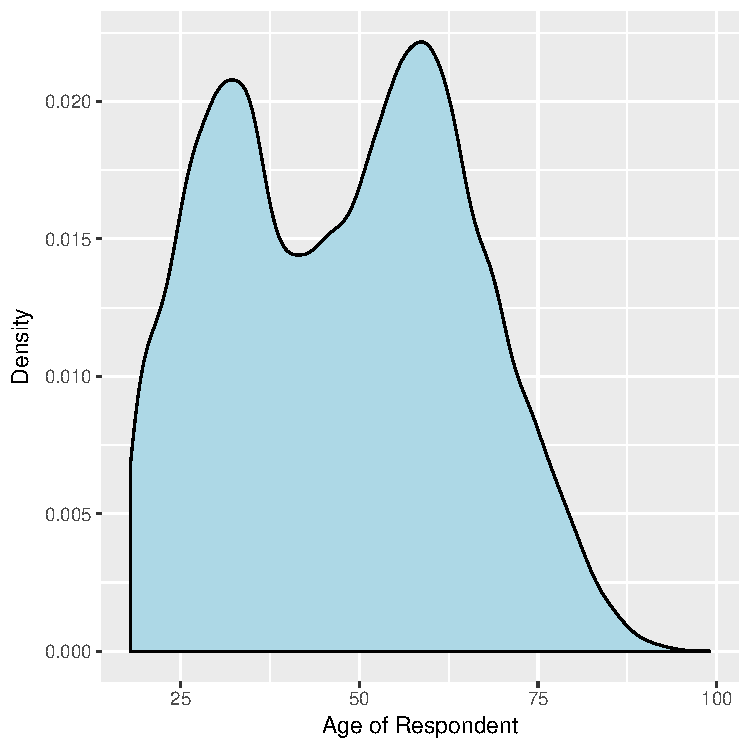
\includegraphics[width=.9\linewidth]{age_density.pdf}
  \caption{Density Plot}
  \label{fig:sub2}
\end{subfigure}
\label{fig:test}
\end{figure}





\newpage
\section{Modeling}
\subsection{OLS Regression}
\begin{lstlisting}
## OLS Regression
# Prepare Obama approval as the DV
cces16$oa <- cces16$CC16_320a
cces16$oa[cces16$oa=="5"] <- NA
cces16$oa[cces16$oa=="8"] <- NA
cces16$oa <- 5 - cces16$oa
# Fit the OLS model
olsfit <- lm(oa ~ pid + ideology +
             gender + white + edu + age,
             data = cces16)
# Print the model summary
summary(olsfit)

Call:
lm(formula = oa ~ pid + ideology + gender + white + edu + age, 
    data = cces16)

Residuals:
<Labelled double>
    Min      1Q  Median      3Q     Max 
-2.9182 -0.4282 -0.0995  0.5670  3.4652 

Coefficients:
              Estimate Std. Error  t value Pr(>|t|)    
(Intercept)  3.5857187  0.0229650  156.139  < 2e-16 ***
pid         -0.8320592  0.0046920 -177.334  < 2e-16 ***
ideology     0.2180571  0.0038937   56.003  < 2e-16 ***
gender      -0.0514957  0.0067446   -7.635 2.29e-14 ***
white       -0.1420162  0.0062221  -22.824  < 2e-16 ***
edu          0.0450144  0.0023178   19.421  < 2e-16 ***
age         -0.0047770  0.0002035  -23.472  < 2e-16 ***
---
Signif. codes:  0 `***` 0.001 `**` 0.01 `*` 0.05 `.` 0.1 ` ` 1

Residual standard error: 0.7994 on 57165 degrees of freedom
  (7428 observations deleted due to missingness)
Multiple R-squared:  0.594,	Adjusted R-squared:  0.594 
F-statistic: 1.394e+04 on 6 and 57165 DF,  p-value: < 2.2e-16
\end{lstlisting}

\newpage
\subsection{Logistic Regression}
\begin{lstlisting}
## Logistic Regression
# Prepare preference for AR ban as DV
cces16$ban_ar <- cces16$CC16_330d
cces16$ban_ar[cces16$ban_ar==2] <- 0
cces16$ban_ar[cces16$ban_ar==8] <- NA
cces16$ban_ar[cces16$ban_ar==9] <- NA
# Fit the logit model
lfit <- glm(ban_ar ~ pid + agecats + edu + 
             gender + white + ideology,
           data=cces16, family = binomial())
# Print the model summary
summary(lfit)

Call:
glm(formula = ban_ar ~ pid + agecats + edu + gender + white + 
    ideology, family = binomial(), data = cces16)

Deviance Residuals: 
    Min       1Q   Median       3Q      Max  
-2.6730  -0.8953   0.4643   0.7626   2.1389  

Coefficients:
                 Estimate Std. Error z value Pr(>|z|)    
(Intercept)      0.479470   0.062011   7.732 1.06e-14 ***
pid             -0.764097   0.013481 -56.678  < 2e-16 ***
agecats36 to 50  0.348234   0.028295  12.307  < 2e-16 ***
agecatsOver 50   0.787903   0.024658  31.953  < 2e-16 ***
edu              0.096402   0.007027  13.719  < 2e-16 ***
gender          -0.933141   0.020543 -45.423  < 2e-16 ***
white           -0.023337   0.018977  -1.230    0.219    
ideology         0.492440   0.012057  40.842  < 2e-16 ***
---
Signif. codes:  0 `***` 0.001 `**` 0.01 `*` 0.05 `.` 0.1 ` ` 1

(Dispersion parameter for binomial family taken to be 1)

    Null deviance: 74291  on 58396  degrees of freedom
Residual deviance: 59454  on 58389  degrees of freedom
  (6203 observations deleted due to missingness)
AIC: 59470

Number of Fisher Scoring iterations: 4
\end{lstlisting}

\newpage
\subsection{Ordinal Logistic Regression}
\begin{lstlisting}
## Ordinal Logistic Regression
# Convert Obama approval to a factor
cces16$oaf <- factor(cces16$oa)
library(MASS)
# Fit the ordinal logit model
olfit <- polr(oaf ~ pid + ideology +
                gender + white + edu + age,
              data = cces16, Hess = TRUE)
# Print the model summary
summary(olfit)

Call:
polr(formula = oaf ~ pid + ideology + gender + white + edu + 
    age, data = cces16, Hess = TRUE)

Coefficients:
             Value Std. Error  t value
pid      -1.677610  0.0136729 -122.696
ideology  0.537569  0.0104278   51.552
gender   -0.156796  0.0175791   -8.919
white    -0.366697  0.0174166  -21.054
edu       0.106201  0.0060308   17.610
age      -0.009955  0.0005329  -18.681

Intercepts:
    Value     Std. Error t value  
1|2   -3.0589    0.0613   -49.9253
2|3   -2.1221    0.0599   -35.4338
3|4   -0.3256    0.0587    -5.5420

Residual Deviance: 106440.27 
AIC: 106458.27 
(7428 observations deleted due to missingness)
\end{lstlisting}

\newpage

\subsection{Multinomial Logistic Regression}
\begin{lstlisting}
## Multinomial Logistic Regression
## Create a 2012 vote choice factor variable
cces16$vc <- cces16$CC16_326
cces16$vc[cces16$vc=="4"] <- NA
cces16$vc[cces16$vc=="5"] <- NA
cces16$vc <- factor(cces16$vc,
                    levels = c(1,2,3),
                    labels = c("Obama", "Romney","Other"))

library(nnet)
# Fit the multinomial logit model
mlfit <- multinom(vc ~ pid + agecats + edu + 
                    gender + white + ideology,
                  data=cces16)
# weights:  27 (16 variable)
initial  value 50436.191560 
iter  10 value 22736.899646
iter  20 value 17517.395617
iter  30 value 16746.999000
final  value 16746.972242 
converged
# Print the model summary
summary(mlfit)
# Note: multinomial logit output omitted here for formatting
\end{lstlisting}

\newpage

\section{\texttt{survey} Package}
All examples in this section require the \texttt{survey} package:
\begin{lstlisting}
library(survey)
\end{lstlisting}

\subsection{Weighted Tabulations}
\begin{lstlisting}
## WITHOUT WEIGHTING 
# Tabulate PID
prop.table(table(cces16$pid_reverse))

# Tabulate PID by age categories
pidxage <- table(cces16$pid_reverse, cces16$agecats)
pidxage
prop.table(pidxage,2)

## WITH WEIGHTING
# Create a survey design dataframe
svy.cces16 <- svydesign(ids = ~1, 
                        data = cces16, 
                        weights = cces16$commonweight_vv)
# Weighted tabulation of PID
prop.table(svytable(~cces16$pid_reverse, design = svy.cces16))

# Weighted tabulation of PID by age categories
prop.table(svytable(~cces16$pid_reverse+cces16$agecats, 
                    design = svy.cces16),2)
\end{lstlisting}

\subsection{Weighted Models}
\begin{lstlisting}
## WITHOUT WEIGHTING 
# Run a logit regression for attitudes toward gun control
fit <- glm(ban_ar ~ pid_reverse + agecats + edu + 
             gender + white + ideology,
           data=cces16, family = binomial())
summary(fit)

## WITH WEIGHTING
wfit <- svyglm(ban_ar ~ pid_reverse + agecats + edu + 
                 gender + white + ideology,
               design=svy.cces16, family = binomial())
summary(wfit)
\end{lstlisting}

\newpage

\subsection{Creating Post-Stratification Weights}
For this example, we will mirror the process I used to generate post-stratification weights for the subsample from the 2016 CCES.

\end{document}
              